\documentclass[]{article}

\usepackage{cite}
\usepackage{amsmath}
\usepackage[letterpaper, margin = 1in]{geometry}
\usepackage{graphicx}

\newcommand\nt{\textup{\scriptsize{0}}}
\newcommand\total{\textup{\scriptsize{total}}}
\newcommand\el{\textup{\scriptsize{el}}}
\newcommand\inel{\textup{\scriptsize{inel}}}
\newcommand\elin{\textup{\scriptsize{el,in}}}
\newcommand\inelin{\textup{\scriptsize{inel,in}}}
\newcommand\out{\textup{\scriptsize{out}}}
\newcommand\PI{\textup{\scriptsize{PI}}}
\newcommand\noscat{\textup{\scriptsize{noscat}}}
\newcommand\sel{\textup{\scriptsize{1el}}}
\newcommand\elpl{\textup{\scriptsize{el,plural}}}
\newcommand\innoinel{\textup{\scriptsize{in,noinel}}}
\newcommand\signal{\textup{\scriptsize{signal}}}
\newcommand\inelpc{\textup{\scriptsize{inel,pc}}}
\newcommand\elplpc{\textup{\scriptsize{el,plural,pc}}}


\title{X-ray microscopy for thick biological specimens}

\begin{document}

\maketitle

\begin{abstract}

\end{abstract}

\section{Introduction}

\section{X-ray interactions}

\paragraph{} The probability for a photon-matter interaction event (either scattering or photoionization) to occur over a fractional penetration depth d\textit{t} can be expressed as
\begin{equation}
P = \sigma_{i} \rho dt
\end{equation}
where $\sigma_{i}$ is the scattering cross section for interaction event \textit{i}, and $\rho$ is the sample density. This report is concerned with interaction events subdivided into elastic scattering, inelastic scattering, and photoionization, with their cross sections respectively represented by $\sigma_{\el}$, $\sigma_{\inel}$, and $\sigma_{\PI}$. To tidy up the narrative, we also denote
\begin{equation}
K_{\el} = \sigma_{\el}\rho
\end{equation}
\begin{equation}
K_{\inel} = \sigma_{\inel}\rho
\end{equation}
\begin{equation}
K_{\elin} = \sigma_{\el}(1-\eta)\rho
\end{equation}
\begin{equation}
K_{\inelin} = \sigma_{\inel}(1-\eta)\rho
\label{eq:inelin}
\end{equation}
\begin{equation}
K_{\out} = \sigma_{\el}\eta\rho + \sigma_{\inel}\eta\rho
\end{equation}
\begin{equation}
K_{\PI} = \sigma_{\PI}\rho
\end{equation}
where $\eta$ is the probability that a photon is backscattered (and thus becomes undetectable) in an elastic scattering event. The spatial distribution of scattered X-ray is given by the atomic form factor
\begin{equation}
F(\theta, \phi) = -\tilde{f}r_e\sqrt{1-\textup{sin}^2\theta \textup{cos}^2\phi}.
\end{equation}
For soft X-ray the angular dependence of scattering factor $\tilde{f}$ is negligible \cite{Lonsdale:1962gz}; moreover, since the square root factor is symmetric in space, $\eta$ can be safely evaluated as 0.5 for elastic scattering. Assuming that inelastic scatterings are isotropic, the same evaluation can be applied to $\eta$ in Equation \ref{eq:inelin}. A series of differential equations of X-ray intensity in various categories as a function of penetration depth $t$ can thereby be written \cite{Jacobsen:1998vj}:

\begin{itemize}

\item The intensity component due to photons that do not undergo any interaction with the sample, $I_{\noscat}$, is given according to
\begin{equation}
dI_{\noscat} = -I_{\noscat}(K_{\inel}+K_{\el}+K_{\PI}) dt.
\end{equation}
with initial condition $I_{\noscat}$(0) = $I_{\nt}$.

\item The component of photons that undergo only one elastic scattering event and remain in the detectable angular range, $I_{\sel}$, is given according to
\begin{equation}
dI_{\sel} = I_{\noscat}K_{\elin} dt - I_{\sel}(K_{\inel}+K_{\el}+K_{\PI}) dt
\end{equation}
with $I_{\sel}$(0) = 0.

\item For the component corresponding to photons undergoing multiple elastic scattering events yet still detectable, $I_{\elpl}$, the differential equation is
\begin{equation}
dI_{\elpl} = I_{\sel}K_{\elin} dt - I_{\elpl}(K_{\out}+K_{\inelin}+K_{\PI}) dt
\end{equation}
with $I_{\elpl}$(0) = 0.

\item For photons that are scattered out of the detectable angular range (backscattered), either elastically or inelastically, the corresponding intensity contribution $I_{\out}$ satisfies
\begin{equation}
dI_{\out} = (I_{\nt} - I_{\out} - I_{\PI})K_{\out} dt
\end{equation}
with $I_{\out}$(0) = 0.

\item For photons that are absorbed via photoionization, the component $I_{\PI}$ satisfies
\begin{equation}
dI_{\PI} = (I_{\nt} - I_{\out} - I_{\PI})K_{\PI} dt
\end{equation}
with $I_{\PI}$(0) = 0.

\item The portion of detectable photons that do not undergo inelastic scattering, i.e., the summation of $I_{\noscat}$, $I_{\sel}$, and $I_{\elpl}$, is denoted as $I_{\innoinel}$ and given by
\begin{equation}
dI_{\innoinel} = -I_{\innoinel}(K_{\inelin}+K_{\out}+K_{\PI})
\end{equation}

\item Lastly, $I_{\inel}$, the contribution of photons that undergo at least one inelastic scattering yet are still within the detectable angular range, is given in
\begin{equation}
dI_{\inel} = I_{\innoinel}K_{\inel} dt - I_{\inel}(K_{\out}+K_{\PI}) dt
\end{equation}
with $I_{\inel}$(0) = 0.

\end{itemize}

\begin{figure}[!b]
\begin{center}
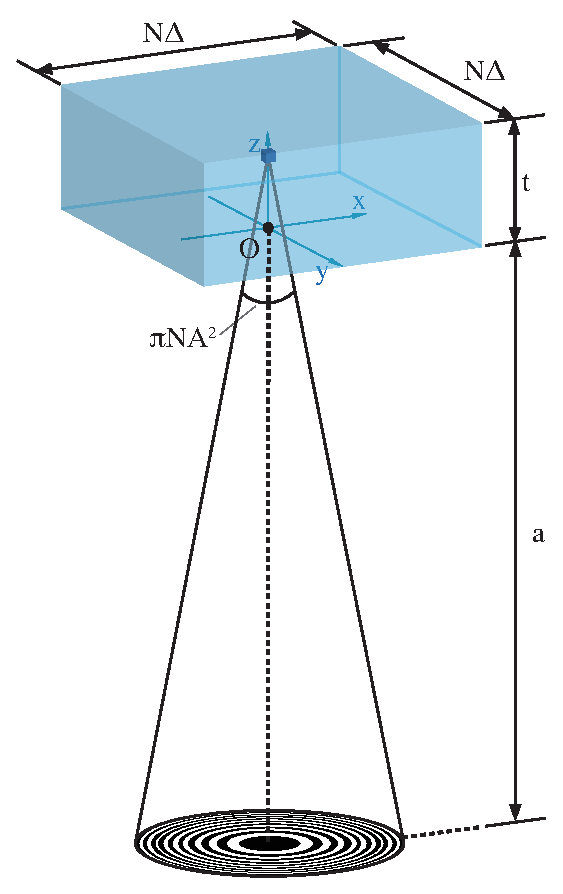
\includegraphics[scale=.6]{epsilon.eps}
\caption{Illustration of the geometric model used for calculating $\epsilon$ for a sample with thickness $t$ and an imaging system with pixel size \textit{$\Delta$}, dimension of field of view $N$, and working distance $a$.}
\label{fig:model}
\end{center}
\end{figure}

\paragraph{} Solutions to these differential equations yield
\begin{equation}
I_{\noscat} = I_{\nt}e^{-(K_{\inel}+K_{\el}+K_{\PI})t}
\end{equation}
\begin{equation}
\begin{aligned}
I_{\sel} &= I_{\nt}K_{\elin}e^{-(K_{\inel}+K_{\el}+K_{\PI})t} \\ &= K_{\elin}tI_{\noscat}
\end{aligned}
\end{equation}
\begin{equation}
I_{\elpl} = I_{\nt} \Big[ e^{-(K_{\out}+K_{\inelin}+K_{\PI})t} - (1+K_{\elin}t)e^{-(K_{\inel}+K_{\el}+K_{\PI})t} \Big]
\end{equation}
\begin{equation}
I_{\out} = \frac{I_{\nt}K_{\out}}{K_{\out}+K_{\PI}} \Big(1 - e^{-(K_{\out}+K_{\PI})t}\Big)
\end{equation}
\begin{equation}
I_{\PI} = \frac{I_{\nt}K_{\PI}}{K_{\out}+K_{\PI}} \Big(1 - e^{-(K_{\out}+K_{\PI})t}\Big)
\end{equation}
\begin{equation}
I_{\innoinel} = I_{\nt}e^{-(K_{\inelin}+K_{\out}+K_{\PI})t}
\end{equation}
\begin{equation}
I_{\inel} = I_{\nt}\Big[e^{-(K_{\out}+K_{\PI})t} - e^{-(K_{\inelin}+K_{\out}+K_{\PI})t)}\Big].
\end{equation}

\paragraph{} In the specific case of X-ray phase contrast imaging, more useful categories can be lined out based on the above results. Taking the interfering amplitudes of $I_{\noscat}$ and $I_{\sel}$ yields the signal intensity:
\begin{equation}
I_{\signal} = \sqrt{I_{\noscat}I_{\sel}}.
\end{equation}

Moreover, if one assumes that inelastic and plural elastic scattering events completely randomize the direction of photons, then the intensity of photons of such kinds that enters the object imaging system and thus contribute to the background of phase contrast imaging, $I_{\inelpc}$ and $I_{\elplpc}$, can be obtained by simply multiplying $I_{\inel}$ and $I_{\elpl}$ by a probability factor $\epsilon$, which is determined purely on geometric basis. The following analysis is applied in calculating the value of $\epsilon$. Consider the region of the sample that is within the instrument's field of view (Figure \ref{fig:model}). For a voxel d$V$ within the volume of interest, the fraction of photons entering the imaging system with numerical aperture $N.A.$ within $I_{\inel}$ or $I_{\elpl}$ is obviously the ratio between $\Omega$, the solid angle of the slanted cone defined by the segments connecting the voxel and the rim of the aperture, and 2$\pi$. If the working distance $a$ is significantly larger than the lateral dimension of the field of view $N\Delta$, where $\Delta$ is the pixel size and $N$ is the number of pixels in the lateral direction, then $\Omega$ can be approximated using the formula for the apex solid angle of an upright cone
\begin{equation}
\Omega = 2\pi(1-\cos\theta)
\end{equation}
where $\theta$ is the average of the apex angles of the triangles cut out from the cone by two orthogonal planes both passing the apex and the bottom center of the cone, one parallel to the slanting direction and the other intersecting with it. The value of $\theta$ can be derived from the coordinates of the voxel as well as $a$ and the aperture radius, $2a(N.A.)$. Then $\epsilon$ can be expressed by
\begin{equation}
\epsilon = \int_V \frac{1}{V} \frac{\Omega(x,y,z)}{2\pi} dV
\end{equation}
where $V$ is the volume of interest. 

\begin{figure}[!t]
\begin{center}
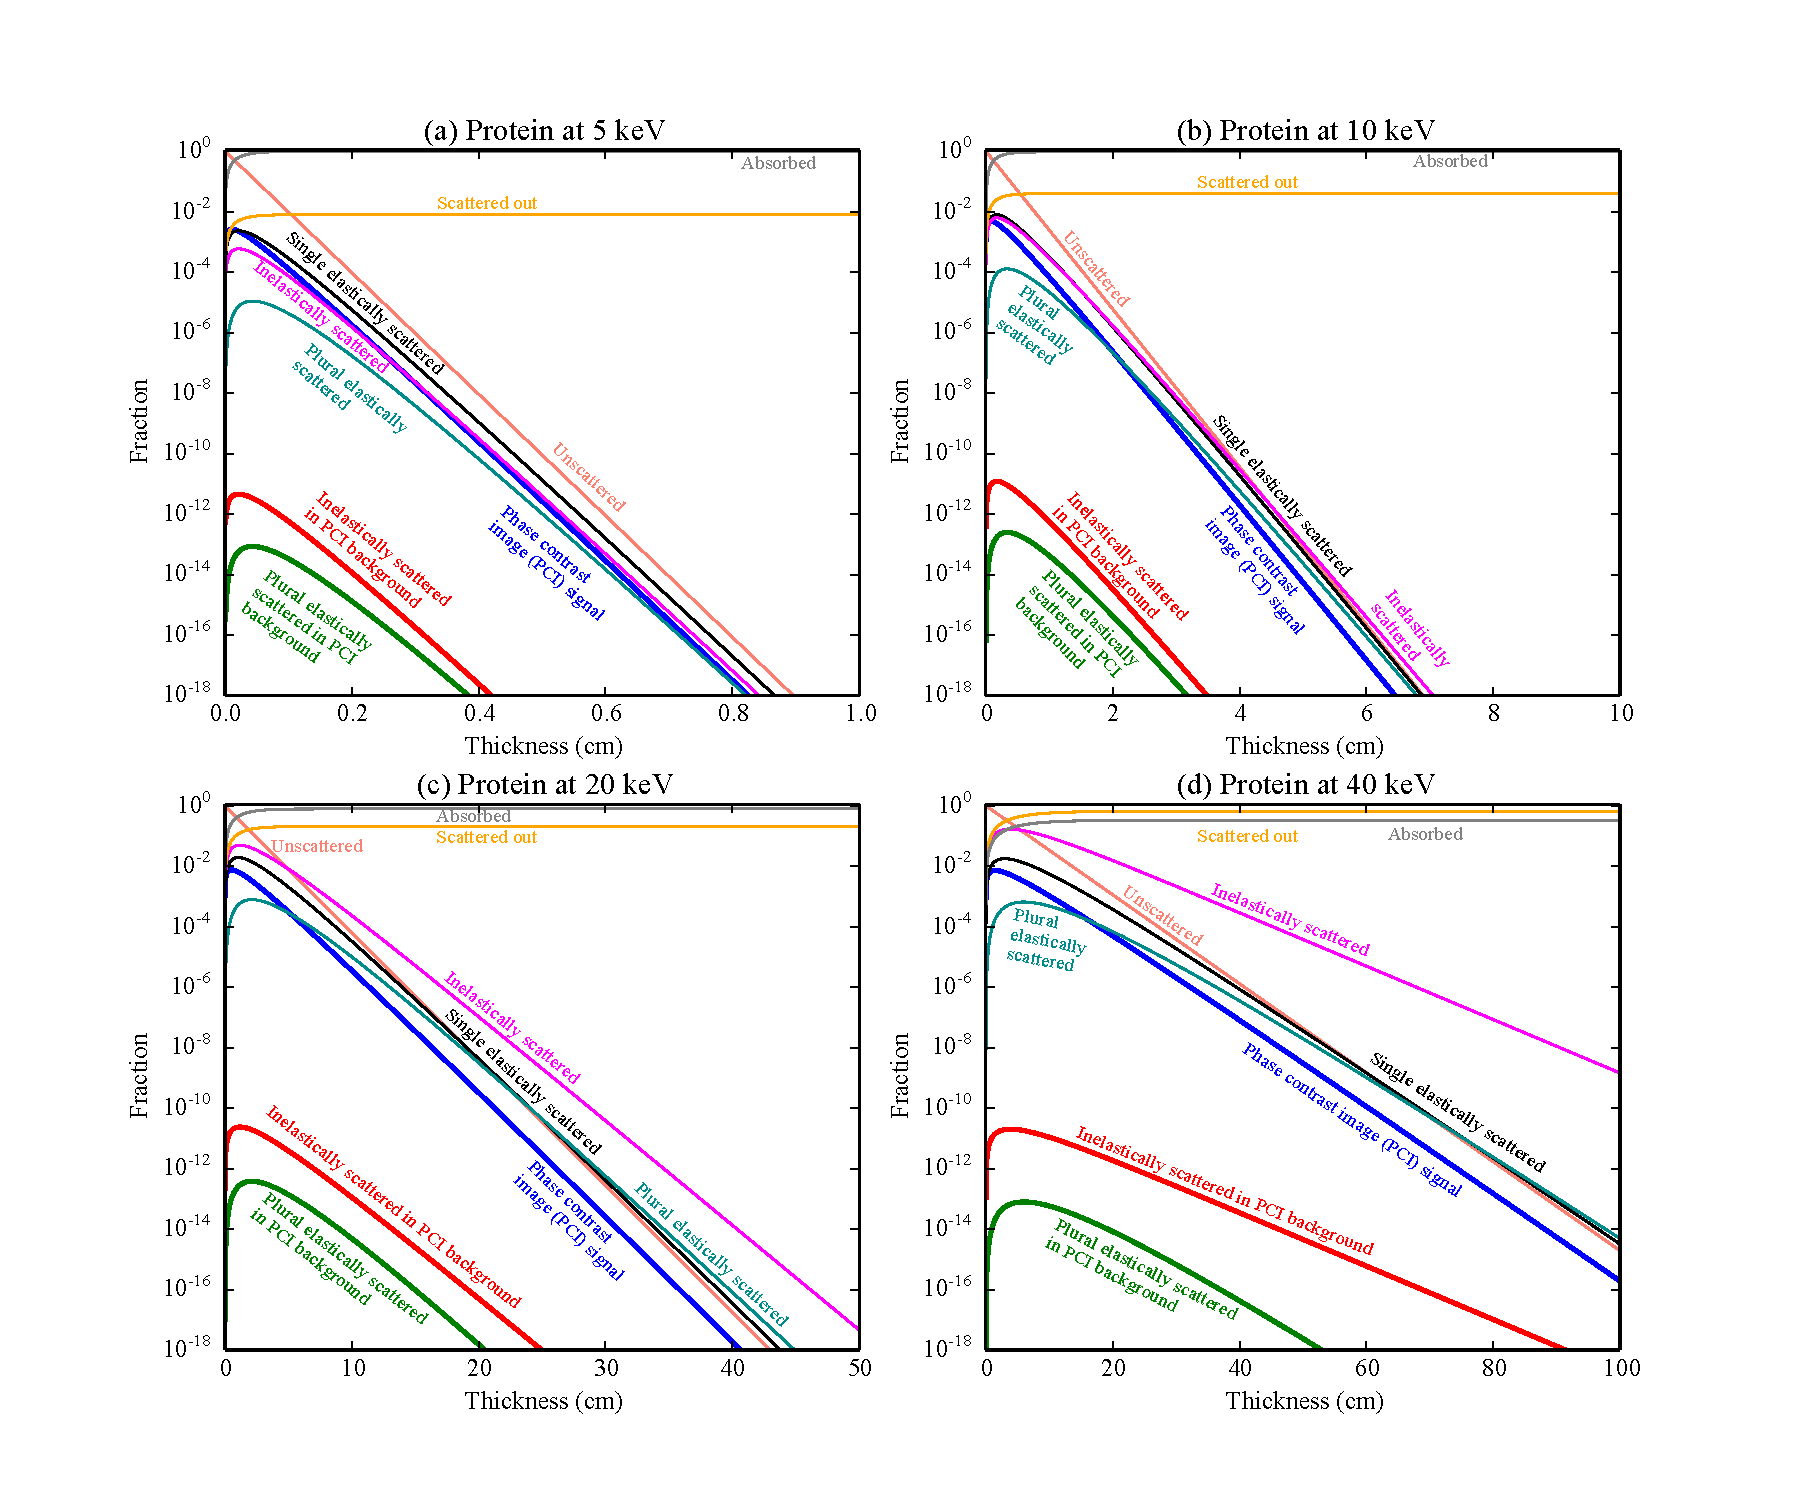
\includegraphics[scale=.53]{unimatrix_fig.eps}
\caption{Normalized intensity profiles for X-ray in protein as a function of thickness at incident energy of (a) 5 keV, (b) 10 keV, (c) 20 keV, and (d) 40 keV. Simulation was run for a typical imaging system where $\Delta$ = 1 $\mu$m, $N$ = 1024, and $a$ = 10 mm.}
\label{fig:unimatrix_inten}
\end{center}
\end{figure}



\paragraph{} Figure \ref{fig:unimatrix_inten} shows the intensity profiles relative to sample thickness at varying energies. 

\bibliography{mybib}{}
\bibliographystyle{ieeetr}

\end{document}